\documentclass{elsart}
\usepackage{amsmath,amssymb}
\usepackage{epsfig}
\usepackage{cite}
\usepackage{fancybox}
\usepackage{multicol}
\usepackage{graphicx}



\bibliographystyle{unsrt}
\journal{Applied Numerical Mathematics}



\psfigdriver{dvips}
\setlength{\oddsidemargin}{-0.06in}

\setlength{\evensidemargin}{0.06in}
\setlength{\topmargin}{0.4in}
\setlength{\textwidth}{6.50in}
\setlength{\textheight}{8.93in}
\raggedbottom \hfuzz=3pt
%

\long\def\comment#1{}
\def \pder#1#2{\frac{\partial {#1}}{\partial {#2}}}
\def \dfe {\buildrel \rm def \over =}
\def\half{{\textstyle {1\over2}}}



% ++++ Vectors.

%  +++++ Tensors
\def \tnsrsig{ \underset{\thickapprox}{\boldsymbol{\sigma} }}
\def \tnsreps{\underset{\thickapprox}{\boldsymbol{\varepsilon} }}




\def\calR{\cal R }

%%%%%%%%%%%%%%%%%%%%%%%%%%%%%%%%%%%%%%%%%%%%%%%%%%%%%%%%%%%%%%%%%%%%%%
% New definitions and commands
\newtheorem{define}{Definition}[section]
\newtheorem{theorem}[define]{Theorem}
\newtheorem{question}[define]{Question}
\newtheorem{problem}[define]{Problem}


%**************************************

\begin{document}
\begin{frontmatter}
\title{Solving ECG Inverse Problems Using Spectral Element Methods}


\author[addr1]{S.\ Choe},
\ead{skchoe@cs.utah.edu}
\author[addr1]{R.\ M.\ Kirby \thanksref{corresp}}
\ead{kirby@cs.utah.edu}


\address[addr1]{School of Computing, Univ.\ of Utah, Salt Lake City, Utah, USA.}

\thanks[corresp]{Corresponding Author}
\date{Dec 1, 2003}


\begin{abstract}

\end{abstract}

\end{frontmatter}

\maketitle
\noindent {\bf Keywords:}

%\tableofcontents



\section{Introduction}
%
%\{ {\it  sp1d\_ch1.tex} \}

Spectral method is a numerical scheme to approximate and simulate the solution of partial differential equations. It have developed rapidly in the past three decades and applied to many field in numerical simulation.

One of main reason for it can gain broad and fast feasibility is that it can take various system of infinitely differentiable basis functions as trial functions. By choosing appropriate orthogonal system based on its domain of orthogonality, we can apply the method to problems such as periodic/non-periodic problems and problems defined on compact domain, half/all intervals.

The other thing which is so fascinating is in its high accuracy. In particular, the spectral polynomial method facilitates to control the resolution of element size and the order of approximation. This enables the method to converge exponential speed which shows a noticeable difference from classical finite difference and element methods.

The goal of this project is to study the fundamental theory of spectral method in its existence, solvability, and obtain its constructive procedure to apply the method in various application field. By checking the solutions of problems having exact solution in its accuracy, we can validate the method and see how much we can save the effort on discretisation of domain to achieve the same degree of accuracy in comparison to classical methods.

In this report, I investigate the spectral method for solving a partial differential equation specific to the forward Poisson problem with Dirichlet and Neumann boundary condition on each end of one dimensional interval domain. Throughout the report, I will briefly explain the method of weighted residual that is necessary to go further toward spectral polynomial method in this section. We will look into mathematical background and procedure of spectral method on forward poisson problem in section 2 and in the end, we make sure the result based on the mathematical theory.


\subsection{Poisson Equations}

In the science and engineering system, we are interested in the system having continuous quantities and relations. We put our main focus on the system having poisson relationship. We have experienced this system in various field such as Electrostatics, Magnetics, Heat flow, Elastic Membranes, Torsion, and Fluid Flow, etc.

For example, in Electrostatics, we can see the Gauss's law in differential form as follows\cite{Johnson}:
\begin{equation}
\nabla \cdot \mathbf{E} = 4 \pi \rho
\end{equation}
which means the charge within a closed spherical surface is related to the electric field \textbf{E} normal to surface element where $\rho$ is a charge density.

Since it is known in electrostatics that the electric field \textbf{E} is conservative, \textbf{E} is a form of gradient of a scalar potential $\Phi$,
\begin{equation}
\mathbf{E} = - \nabla\Phi.
\end{equation}
With these two relationships, we obtain a Poisson equation
\begin{equation}
\nabla^2\Phi = -4\pi\rho.
\end{equation}

In this report, the Poisson equation is defined as

\begin{equation}
\label{poisson1}
L(u) \equiv  \nabla^2 u + f = 0.
\end{equation}
where $u$ and $f$ are defined on $\Omega$.

In pointwise viewpoint, the one dimensional Poisson equation
(\ref{poisson1}) is written as
\begin{equation}
\label{poisson2}
L(u)(x) \equiv \frac{d^2}{dx^2} u(x) + f(x) = 0,
\end{equation}
for all $x$ in $[a, b]$.

\subsection{Method of Weighted Residuals}
Accroding to the Weierstrass approximation theorem, for any given real valued continuous solution $u$ on a compact interval $[a, b]$ we can obtain real polynomial function $p$ of certain degree such that $p$ uniformly approximates $u$. Even though the speed of convergence of each point are within a predefined bandwidth this doesn't satisfies the requirement that we need to acquire an accurate solution on some specific situatation. By imposing certain restriction, we can get the formularation that satifies the requirement.

To describe this, we set a general linear differential equation on $\Omega$.
\begin{equation}
\label{pde1} L(u) = 0.
\end{equation}
with appropriate initial and boundary conditions. Under certain restriction, we assume that the solution $u(x)$ can be represented exactly in the form of approximation
\begin{equation}
\label{sol1} u^{\delta}(x) = \sum_{i=0}^{N_{dof-1}} \hat u_i \Phi_i(x),
\end{equation}
where $\Phi_i(x)$ are polynomials called trial functions and $\hat u_i$ are $N_{dof}$ unknown coefficients by assuming the following:
\begin{eqnarray}
        \hat u_0  &=& \mathcal{G}_{D} \qquad \mbox{: Dirichlet Boundary Value}, \\
        \Phi_0(x) &=& 1, \qquad \mbox{where we define Dirichlet condition on }\partial\Omega, \mbox{ and}\\
    \Phi_i(\partial\Omega) &=& 0, \qquad i \ge 1.
\end{eqnarray}
Then we can define a non-zero residual $R$ by
\begin{equation}
R(u^{\delta}) = L(u^{\delta}).
\end{equation}

We define an innner-product $\langle \cdot, \cdot \rangle$ over $C^0(\Omega)$  as follows:
\begin{equation}
\label{functional}
\langle u, v \rangle = \int_{\Omega} u(x) \cdot v(x) dx.
\end{equation}

The restriction of this method is imposed on the choice of test function $v(x)$ that satisfies
\begin{equation}
\langle v, R \rangle = 0.
\end{equation}

For example, in the collocation method, the $j^{th}$ test function is the Dirac delta function which is one at a collocation point $x = x_j$. Then we have
\begin{equation}
0 = \langle \delta_j, R \rangle = \int_{\Omega} R(u^{\delta})(x)\delta_j(x)dx = R(u^{\delta})(x_j) = L(u^{\delta})(x_j).
\end{equation}

Other types of test functions are explaned in \cite{Karniadarkis} with the list of test functions that we can characterize the restrictions based on their definition. The Galerkin method is one such method in which the test functions are defined by $\Phi_i$ which are in the same set of trial functions.


\section{Theory of Spectral Polynomial/Fourier Elements Method}
%%\{ {\it  sp1d\_ch2.tex} \}

To formulate Spectral Element Methods, we presume the following boundary conditions to the equation (\ref{poisson1}) and (\ref{poisson2}).
\begin{eqnarray}\label{bdycond}
    u(a) &=& {\mathcal G}_D \qquad \mbox{ : Dirichlet Condition}\\
    \frac{d}{dx}u(b) &=& \mathcal{G}_N \qquad \mbox{ : Neumann Condition}.
\end{eqnarray}

Multiplying equation (\ref{poisson1}) and by integration by part,
\begin{eqnarray}
\int_a^b v(x)\frac{d^2}{dx^2}u(x) dx &+& \int_a^b v(x) f(x) dx = 0,\\
\label{weakform1}
\int_a^b \frac{d}{dx}v(x)\frac{d}{dx}u(x)dx &=& \int_a^b v(x) f(x) dx + \left[v \frac{d}{dx}u\right]_a^b,
\end{eqnarray}
for $u, v$ being sufficiently smooth.

Define a set $H^1(\Omega)$ of functions and a norm $||\cdot||_{H^1(\Omega)}$ on it as follows:
\begin{eqnarray}
H^1(\Omega) &=& \{v \in L^2(\Omega) : \frac{d}{dx}v \in L^2(\Omega)\}, \\
||v ||_{H^1(\Omega)} &=& \left[ \int_{\Omega}v(x)^2 + \frac{d}{dx}v(x)^2 dx \right]^{\frac{1}{2}}, \quad v \in H^1(\Omega).
\end{eqnarray}

Consider solutions to problem (\ref{poisson1}) where the forcing function $f$ is well defined in the sense that
$\int_a^b v f + \left[ v u^{\prime} \right]_a^b < \infty$. Therefore we only consider trial solutions to equation (\ref{weakform1}) which lie in $H^1(\Omega)$ and satisfy the Dirichlet boundary condition. We can define the trial space by

\begin{equation}
\mathcal{X} = \{u\in H^1|u(a) = {\mathcal G}_D\}.
\end{equation}
Similarly, the space of all test functions are defined by being homogeneous on all Dirichlet boundaries, that is
\begin{equation}
\mathcal{V} = \{v\in H^1|v(a) = 0\}.
\end{equation}

For numerical approximation, we select finite subspace $\mathcal{X}^{\delta} (\subset \mathcal{X})$ and $\mathcal{V}^{\delta} (\subset \mathcal{V})$ for which equation (\ref{weakform1}) holds. In particular, we can define $\delta$ by the choice of two different discretization approaches : Element size or Polynomial order. The formulation for the weak solution (\ref{weakform1}) can be stated as:

Find $u^{\delta} \in \mathcal{X}^{\delta}$, such that
\begin{equation}
\int_a^b \frac{d}{dx}v^{\delta}(x)\frac{d}{dx}u^{\delta}(x)dx = \int_a^b v^{\delta}(x) f(x) dx + \left[v^{\delta} \frac{d}{dx}u^{\delta}\right]_a^b, \qquad v^{\delta} \in \mathcal{V}^{\delta}.
\end{equation}




%we find $u^{\delta}$ such that

%\begin{equation}
%\label{weakabs}
%\langle L(u), v \rangle = \langle \nabla^2 u, v \rangle + \langle f, v \rangle =\int_a^b \frac{d^2}{dx^2} u(x) v(x) dx + \int_a^b f(x) v(x) dx = 0,
%\end{equation}
%where by the definition of Galerkin method, $v$ is function generated by linear combination from a set of basis functions on which $u$ defined in $\left[a, b\right]$.

%--------------------------------------------------------------------------
\subsection{Basis Functions}

The spectral approximation of solution $u$ is generally represented as
\begin{equation}\label{genrep}
u(x) = \sum_{i=0}^{N_{dof-1}} \hat u_i\Phi_i(x)
\end{equation}
on $[a, b]$. To construct the global basis functions $\{\Phi_i(x)\}_{i=0}^{N_{dof-1}}$, each $\Phi_i$ is represented by the linear combination of local basis functions $\phi_i$ on each element in $[a, b]$, say $\Omega^e$.

We define the local basis functions ${\phi_i}$ on $[-1, 1]$ to be a real valued function with Jacobi polynomial of $\alpha = 1$ and $\beta = 1$ $\{P_i^{1,1}\}$ as follows:
\begin{equation}
\label{locbasis}
  \phi_i(\xi) =\left \{
    \begin{array}{ll}
    \frac{1-\xi}{2}, & i=0 \\
    \left(\frac{1-\xi}{2}\right)\left(\frac{1+\xi}{2}\right)P_{i-1}^{1,1}(\xi),
    \qquad &1 \le i \le P-1 \\
    \frac{1+\xi}{2}, & i=P \\
    \end{array}   \right.
\end{equation}
for all $\xi$ in $[-1, 1]$.

Then on a single standard element $[-1, 1]$, the approximation $u(\xi)$ is represented as
\begin{equation}\label{locrep}
u(\xi) = \sum_{i=0}^{P_e} \hat u_{i}^{e}\phi_i(\xi),
\end{equation}
for $\xi$ in $[-1, 1]$.

The local basis function $\phi_i^e$ on general element $[x_1, x_2]$ is defined by the change of variable for $\phi_i$ between two interval $[x_1, x_2]$ and $[-1, 1]$.

%--------------------------------------------------------------------------
\subsection{Spectral Polynomial Method in an Element}

We apply the basis representation (\ref{locrep}) to weak formulation (\ref{weakform1}) with the same test function $\{\phi_q\}$, then we obtain the following:
\begin{equation}\label{locmat}
 - \sum_{p=0}^{P_e} \hat u_p^e \langle \frac{d^2}{dx^2} \phi_p, \phi_q \rangle = - \langle \frac{d^2}{dx^2} \sum_{p=0}^{P_e} u_p^e \phi_p, \phi_q \rangle = \langle f, \phi_q \rangle
\end{equation}
for $q = 0, \cdots, P_e$ where $P_e$ is the order of polynomial on local element $\Omega^{e}$, say $\left[ x_1, x_2 \right]$.

By integration by part, we can use the fact that
\begin{equation}\label{intpart}
\langle \frac{d^2}{dx^2} \phi_p, \phi_q \rangle = \left[ \frac{d}{dx}\phi_p(x) \phi_q(x) \right]_{x_1}^{x_2} - \langle \frac{d}{dx} \phi_p, \frac{d}{dx} \phi_q \rangle.
\end{equation}

by applying (\ref{intpart}) to (\ref{locmat}), we obtain
\begin{eqnarray}\label{locmat}
&- \left[\frac{d}{dx}u(x)\phi_q(x) \right]_{x_1}^{x_2} + \sum_{p=0}^{P_e} \hat u_p^e \langle \frac{d}{dx} \phi_p, \frac{d}{dx} \phi_q \rangle
%= - \left[ \sum_{p=0}^{P_e} \hat u_p^e \frac{d}{dx}\phi_p(x) \phi_q(x) \right]_{x_1}^{x_2} + \sum_{p=0}^{P_e} \hat u_p^e \langle \frac{d}{dx} \phi_p, \frac{d}{dx} \phi_q \rangle \\
= - \sum_{p=0}^{P_e} \hat u_p^e \langle \frac{d^2}{dx^2} \phi_p, \phi_q \rangle  = \langle f, \phi_q \rangle \\
&\sum_{p=0}^{P_e} \hat u_p^e \langle \frac{d}{dx} \phi_p, \frac{d}{dx} \phi_q \rangle = \langle f, \phi_q \rangle + \left[\frac{d}{dx}u(x)\phi_q(x) \right]_{x_1}^{x_2}
\end{eqnarray}
for $q = 0, \cdots, P_e$.

In matrix form we obtain the following the system of equations for local coefficients and modes:
Note that $\phi_q(x_1) = \delta_{q,1}$, $\phi_q(x_2) = \delta_{q, P_e}$ and the orthogonality on $\{\phi_q\}_{q=1}^{P_e-1}$ .
\begin{eqnarray}
\label{localsystem}
\begin{bmatrix}
    \phi_{0,0}^e   & 0            & \cdots & 0                    & \phi_{0,P_e}^e      \\
    0              & \phi_{1,1}^e & \cdots & 0                    & 0                   \\
    \vdots         & \vdots       & \ddots & \vdots               & \vdots              \\
    0              & 0            & \cdots & \phi_{P_e-1,P_e-1}^e & 0                   \\
    \phi_{P_e,0}^e & 0            & \cdots & 0                    & \phi_{P_e,P_e}^e    \\
\end{bmatrix}
\begin{bmatrix}
    {\hat u^e}_{0}      \\
    {\hat u^e}_{1}      \\
    \vdots              \\
    {\hat u^e}_{P_e-1}  \\
    {\hat u^e}_{P_e}    \\
\end{bmatrix}
=
\begin{bmatrix}
    f^e_{0}     \\
    f^e_{1}     \\
    \vdots      \\
    f^e_{P_e-1} \\
    f^e_{P_e}   \\
\end{bmatrix}
+
\begin{bmatrix}
    0       \\
    0       \\
    \vdots  \\
    0       \\
    1       \\
%    \phi_{0}(x_2)     \\
%    \phi_{1}(x_2)     \\
%    \vdots            \\
%    \phi_{P_e-1}(x_2) \\
%    \phi_{P_e}(x_2) \\
\end{bmatrix}
u^{\prime}(x_2)
-
\begin{bmatrix}
    1       \\
    0       \\
    \vdots  \\
    0       \\
    0       \\
%    \phi_{0}(x_1)     \\
%    \phi_{1}(x_1)     \\
%    \vdots            \\
%    \phi_{P_e-1}(x_1) \\
%    \phi_{P_e}(x_1) \\
\end{bmatrix}
u^{\prime}(x_1)
\end{eqnarray}
where $\phi_{p,q} = \langle \frac{d}{dx} \phi_p, \frac{d}{dx} \phi_q \rangle$, $f_q^e = \langle f, \phi_q \rangle$, $p, q = 0, \ldots, P_e $.


\subsection{Global Assembly/Direct Stiffness Summation} As seen on
equation (\ref{sol1}), we have the finite element approximation
$u^{\delta}$ in terms of the global modes. Moreover, we can
represent $u^{\delta}$ in terms of linear combination of local
modes ${\phi_p^e}$ :
\begin{equation}
\label{sol2} u^{\delta}(x) = \sum_{i=0}^{N_{dof-1}}\hat u_i \Phi_i(x) = \sum_{e=1}^{N_{el}}\sum_{p=0}^{P_e}{\hat u}_p^e \phi_p^e(\xi),
\end{equation}
where in this case $P_e$ is the polynomial order of the expansion and $\phi_p^e(\xi)$ is reparametrization of local basis function general elements.

We have the following relationship between global and local coefficients $(\hat u_i,\hat u_i^e)$:
\begin{eqnarray}
\label{coefoverlap}
\hat u_0^1 &=& \hat u_0 \\
\hat u_{P_{e}}^{e} &=& \hat u_{0}^{e+1} = \hat u_r, \qquad e = 1, \ldots, N_{el}-1, \mbox{ for some } r \le N_{dof}-2, \mbox{ and}\\
\hat u_{P_{e}}^{e} &=& \hat u_r, \qquad \qquad e = N_{el},\quad r = N_{dof}-1.
\end{eqnarray}

When we determine $\hat u_i, i = 0, \ldots, N_{dof}-1$, this
property plays a role that we can reduce the size of system.

According to the orthogonality defined in $\{\phi_p^e\}$, the following relationships hold
\begin{equation}
\label{q0}\phi_{q,q}^e \hat u_q^e = f_q^e, \qquad q = 1, \ldots, P_e-1
\end{equation}
for every element $e$.

By the orthogonality in $\{\phi_p^e\}$ and the identity (\ref{coefoverlap}) we obtain the relationship below:

For adjacent elements $e_0=[x_0, x_1]$, $e_1=[x_1, x_2]$, and $e_1=[x_2, x_3]$ of polynomial order $P_0, P_1$, and $P_2$, respectively,
\begin{eqnarray}
\label{q1}  \phi_{P_0, 0}^0\hat u_0^0 + \phi_{P_0, P_0}^0 \hat u_{P_0}^0 &=& f_{P_0}^0 - u^{\prime}(x_1) \\
\label{q2}  \phi_{0, 0}^1\hat u_0^1 + \phi_{0, P_1}^1 \hat u_{P_1}^1     &=& f_{0}^1 + u^{\prime}(x_1) \\
\label{q3}  \phi_{P_1, 0}^1\hat u_0^1 + \phi_{P_1, P_1}^1 \hat u_{P_1}^1 &=& f_{P_1}^1 - u^{\prime}(x_2) \\
\label{q4}  \phi_{0, 0}^2\hat u_0^2 + \phi_{0, P_2}^0 \hat u_{P_2}^2     &=& f_{0}^2 + u^{\prime}(x_2)
\end{eqnarray}
(\ref{q1})$+$(\ref{q2}), (\ref{q3})$+$(\ref{q4}) give
\begin{eqnarray}
\label{q5}  -.5 \cdot \hat u_0^0 + 1 \cdot \hat u_{P_0}^0(=u_0^1) -.5 \cdot \hat u_{P_1}^1 &=& f_{P_0}^0 + f_{0}^1 \\
\label{q6}  -.5 \cdot \hat u_0^1 + 1 \cdot \hat u_{P_1}^1(=u_0^2) -.5 \cdot \hat u_{P_2}^2 &=& f_{P_1}^1 + f_{0}^2
\end{eqnarray}

By equation (\ref{q0}),(\ref{q5}), and (\ref{q6}) we can deduce
the system of global stiffness matrix showing the assembly of two
adjacent local element matrix system as follows:
\begin{eqnarray}
\label{localsystem}
&{\mathbf A \mathbf{\hat u} = \mathbf f} \mbox{ is defined by }
\end{eqnarray}
\begin{eqnarray*}
\begin{bmatrix}
    \ddots &\vdots  &\vdots &\vdots &\vdots &\vdots &\vdots &\vdots & \\
    \cdots0 &\phi_{P_0-1,P_0-1}^0   & 0     & 0     &\cdots & 0     & 0     & 0     &0\cdots    \\
    \cdots-.5\cdots0 & 0    & 1     & 0     &\cdots & 0     & -.5   & 0     &0\cdots \\
    \cdots0 & 0      & 0    &\phi_{1,1}^1   &\cdots & 0     & 0     & 0     &0\cdots \\
    \vdots &\vdots  &\vdots &\vdots &\ddots &\vdots &\vdots &\vdots &\vdots  \\
    \cdots0 & 0      & 0    & 0    &\cdots  &\phi_{P_1-1,P_1-1}^1   & 0     & 0   &0\cdots \\
    \cdots0 & 0      & -.5  & 0    &\cdots  & 0     &1      & 0     & 0\cdots-5\cdots \\
    \cdots0 & 0      & 0    & 0    &\cdots  & 0     &0      &\phi_{P_0,P_0}^2   & 0\cdots \\
           &\vdots  &\vdots &\vdots &\vdots &\vdots &\vdots &\vdots &\ddots
\end{bmatrix}
\begin{bmatrix}
    \vdots      \\
    {\hat u_{P_0-1}^0}  \\
    {\hat u_0^1}\\% = {\hat u_{P_0}^0} \\
    {\hat u_1^1}\\
    \vdots      \\
    {\hat u_{P_1-1}^1}  \\
    {\hat u_0^2}\\% = {\hat u_{P_1}^1} \\
    {\hat u_1^2}\\
    \vdots
\end{bmatrix}
=
\begin{bmatrix}
    \vdots      \\
    f_{P_0-1}^0 \\
    f_{P_0}^0 + f_{0}^1 \\
    f_{1}^1 \\
    \vdots  \\
    f_{P_1-1}^1 \\
    f_{P_1}^1 + f_{0}^2 \\
    f_{1}^2 \\
    \vdots
\end{bmatrix}.
\end{eqnarray*}

\subsection{Applying Boundary Conditions}
Now we can apply the boundary conditions defined in (\ref{bdycond}). This is done by processing the system (\ref{localsystem}) about the boundary points $x = a$ and $x = b$. We can apply the idea into the global system as follows:
\begin{eqnarray}
\label{gsystem} {\mathbf A \mathbf{\hat u} = \mathbf f}+
\begin{bmatrix}
    0       \\
    \vdots  \\
    0       \\
    1
\end{bmatrix}
u^{\prime}(b)
-
\begin{bmatrix}
    1       \\
    0       \\
    \vdots  \\
    0
\end{bmatrix}
u^{\prime}(a)
= {\mathbf f}
+
\begin{bmatrix}
    0       \\
    \vdots  \\
    0       \\
    1
\end{bmatrix}
\mathcal{G}_N
-
\begin{bmatrix}
    1       \\
    0       \\
    \vdots  \\
    0
\end{bmatrix}
u^{\prime}(a)
\end{eqnarray}.

Let's set
\begin{equation}
\mathbf{A} =
\begin{bmatrix}
    A_{0,0}         &\cdots     & A_{0,N_{dof}-1}   \\
    \vdots          &\cdots     &\vdots             \\
    A_{N_{dof}-1,0} &\cdots     & A_{N_{dof}-1,N_{dof}-1}
\end{bmatrix},
\qquad
\mathbf{\hat u} =
\begin{bmatrix}
    \hat u_0    \\
    \vdots      \\
    \hat u_{N_{dof}-1}
\end{bmatrix},
\mbox{ and }
\qquad
\mathbf{f} =
\begin{bmatrix}
    f_0    \\
    \vdots \\
    f_{N_{dof}-1}
\end{bmatrix}.
\end{equation}



Since $\hat u_0$ is known to be $\mathcal{G}_D$, we can modify
(\ref{gsystem}) to
\begin{eqnarray}
\label{g2system}
\begin{bmatrix}
    1               & 0         &\cdots     & 0   \\
    A_{1,0}         & A_{1,0}   &\cdots     & A_{1,N_{dof}-1}   \\
    \vdots          &\vdots     &\vdots     &\vdots        \\
    A_{N_{dof}-1,0} & A_{N_{dof}-1,1} &\cdots     & A_{N_{dof}-1,N_{dof}-1}
\end{bmatrix}
\begin{bmatrix}
    \hat u_0    \\
    \hat u_1    \\
    \vdots      \\
    \hat u_{N_{dof}-1}
\end{bmatrix}
=
\begin{bmatrix}
    0       \\
    f_1     \\
    \vdots  \\
    f_{N_{dof}-1}
\end{bmatrix}
+
\begin{bmatrix}
    0       \\
    \vdots  \\
    0       \\
    1
\end{bmatrix}
\mathcal{G}_N
-
\begin{bmatrix}
    -1       \\
    0       \\
    \vdots  \\
    0
\end{bmatrix}
\mathcal{G}_D
\end{eqnarray}

We finally get a system of equations that has solution.

\begin{eqnarray}
\begin{bmatrix}
    1       & 0         &\cdots     & 0   \\
    0       & A_{1,0}   &\cdots     & A_{1,N_{dof}-1}   \\
    \vdots  &\vdots     &\vdots     &\vdots        \\
    0       & A_{N_{dof}-1,1} &\cdots     & A_{N_{dof}-1,N_{dof}-1}
\end{bmatrix}
\begin{bmatrix}
    \hat u_0    \\
    \hat u_1    \\
    \vdots      \\
    \hat u_{N_{dof}-1}
\end{bmatrix}
=
\begin{bmatrix}
    0       \\
    f_1     \\
    \vdots  \\
    f_{N_{dof}-1}
\end{bmatrix}
+
\begin{bmatrix}
    0       \\
    \vdots  \\
    0       \\
    1
\end{bmatrix}
\mathcal{G}_N
-
\begin{bmatrix}
    -1       \\
    A_{1,0}  \\
    \vdots   \\
    A_{N_{dof}-1,0}
\end{bmatrix}
\mathcal{G}_D.
\end{eqnarray}

This solves the system of equation and we obtain $[\hat u_0, \cdots, \hat u_{N_{dof}-1}]^T$.




\{ {\it  sp2d\_ch21.tex} \}

\subsection{2 Dimensional Annulus Problem}

\begin{eqnarray}
- \left(\frac{\partial^2}{\partial r^2} + \frac{1}{r} \frac{\partial}{\partial r} + \frac{1}{r^2}\frac{\partial^2}{\partial \theta^2} \right) u(r,\theta) = f(r,\theta) \\
u(r=a,\theta) = g_1(\theta), \;\; \theta \in [0,2\pi] \\
\frac{\partial}{\partial r} u(r=b,\theta) = 0, \;\; \theta \in [0,2\pi] \\
u(r,\theta=0) = u(r,\theta=2\pi), \;\; r\in[a,b] \\
\int_0^{2\pi} u(r,\theta) d\theta = \mathbf{\int_o^{2\pi} g_1(\theta) d\theta}, \;\; r\in[a,b]
\end{eqnarray}



Assume that $N$ is an even number, $x_j = \frac{2\pi}{N}j, \; j=1,\ldots,N$, then:

\begin{eqnarray}
\hat{u}_k = \frac{1}{2\pi} \int_0^{2\pi}  e^{-ikx} u(x) dx  \simeq \frac{1}{2\pi}\frac{2\pi}{N} \sum_{j=0}^{N-1} e^{-ikx_j} u(x_j),  \;\; k=-\frac{N}{2}+1,\ldots,\frac{N}{2}\\
u_j = u(x_\mathbf{j}) = \sum_{k=-N/2+1}^{N/2} e^{ikx_j}\hat{u}_k, \;\; j=1,\ldots,N.
\end{eqnarray}

We have the orthogonal basis $\{e^{ik\theta}\}_{k = 0}^{N-1}$ with the following orthogonality:
\begin{equation}
\frac{1}{2\pi} \int_{0}^{2\pi} e^{ik\theta} e^{iq\theta} d\theta = \delta_{kq}.
\end{equation}



The representation of $u$ is guaranteed by Weierstrass theorem:
\begin{equation}
u(r,\theta) = \sum_{j=0}^{N_r} \sum_{k=-N_\theta/2+1}^{N_\theta/2} \hat{u}_{jk} \phi_j(r) e^{ik\theta}
\end{equation}

Then the Poisson equation and its modified form of polar coordinate was obtained:
\begin{eqnarray}
- \frac{\partial^2}{\partial r^2}u(r,\theta) - \frac{1}{r} \frac{\partial}{\partial r} u(r,\theta) - \frac{1}{r^2}\frac{\partial^2}{\partial \theta^2} u(r,\theta) &=& f(r,\theta) \\
- r^2 \frac{\partial^2}{\partial r^2} u(r,\theta) - r \frac{\partial}{\partial r} u(r,\theta) - \frac{\partial^2}{\partial \theta^2} u(r,\theta) &=& r^2 f(r,\theta)
\end{eqnarray}


Let us define the following matrices:
\begin{eqnarray}
({\bf M}_1)_{ij} & = & \int_a^b \phi_i(r) \phi_j(r) \;dr  \\
({\bf M}_2)_{ij} & = & \int_a^b r \phi_i(r) \frac{d}{dr} \phi_j(r) \;dr  \\
({\bf M}_3)_{ij} & = & \int_a^b r^2  \frac{d}{dr} \phi_i(r)  \frac{d}{dr} \phi_j(r) \;dr
\end{eqnarray}

To apply Galerkin method, test functions are of the form:
\begin{equation}
\phi_p(r) e^{iq\theta}, \;\; p=0,\ldots,N_r, \;\; q = -\frac{N_\theta}{2}+1,\ldots,\frac{N_\theta}{2}
\end{equation}

We have the weak form of the equation:
\begin{equation}
-\langle  r^2 \frac{\partial^2}{\partial r^2} u(r,\theta) + r \frac{\partial}{\partial r} u(r,\theta) + \frac{\partial^2}{\partial \theta^2} u(r,\theta), \phi_p(r) e^{iq\theta} \rangle = \langle r^2 f(r,\theta), \phi_p(r) e^{iq\theta} \rangle.
\end{equation}

\begin{eqnarray}
&-& \int_a^b \int_0^{2\pi} \phi_p(r) e^{iq\theta} r^2 \frac{\partial^2}{\partial r^2} u(r,\theta) d\theta dr \\
&-& \int_a^b \int_0^{2\pi} \phi_p(r) e^{iq\theta} r \frac{\partial}{\partial r} u(r,\theta) d\theta dr \\
&-& \int_a^b \int_0^{2\pi} \phi_p(r) e^{iq\theta} \frac{\partial^2}{\partial \theta^2} u(r,\theta) d\theta dr  \\
&=& \int_a^b \int_0^{2\pi} \phi_p(r) e^{iq\theta} r^2 f(r,\theta) d\theta dr \\
\end{eqnarray}


\begin{eqnarray}
T_1 &=& \int_a^b \int_0^{2\pi} \phi_p(r) e^{iq\theta} r^2 \frac{\partial^2}{\partial r^2} u(r,\theta) d\theta dr \\
    &=& \int_0^{2\pi} \sum_j \sum_k \hat{u}_{jk} e^{iq\theta} e^{ik\theta} \int_a^b r^2 \frac{d^2}{dr^2} \phi_j(r) \phi_p(r) dr d\theta\\
    &=& \int_0^{2\pi} \sum_j \sum_k \hat{u}_{jk} e^{iq\theta} e^{ik\theta} \left( \left[r^2 \phi_p(r) \frac{d}{dr}\phi_j(r)\right]_a^b -
        \int_a^b \left(2 r \phi_p(r) \frac{d}{dr}\phi_j(r) + r^2 \frac{d}{dr}\phi_p(r) \frac{d}{dr}\phi_j(r)\right) dr \right) d\theta \\
    &=& \int_0^{2\pi} \sum_j \sum_k \hat{u}_{jk} e^{iq\theta} e^{ik\theta} \left( \left[r^2 \phi_p(r) \frac{d}{dr}\phi_j(r)\right]_a^b - 2 ({\bf M}_2)_{pj} - ({\bf M}_3)_{pj} \right) d\theta \\
    &=& 2\pi \sum_j \sum_k \hat{u}_{jk} \delta_{qk} \left( \left[r^2 \phi_p(r) \frac{d}{dr}\phi_j(r)\right]_a^b - 2 ({\bf M}_2)_{pj} - ({\bf M}_3)_{pj} \right)
\end{eqnarray}

\begin{eqnarray}
T_2 &=& \int_a^b \int_0^{2\pi} \phi_p(r) e^{iq\theta} r \frac{\partial}{\partial r} u(r,\theta) d\theta dr \\
    &=& \int_0^{2\pi} \sum_j \sum_k \hat{u}_{jk} e^{iq\theta} e^{ik\theta} \int_a^b r \frac{d}{dr} \phi_j(r) \phi_p(r) dr d\theta\\
    &=& \int_0^{2\pi} \sum_j \sum_k \hat{u}_{jk} e^{iq\theta} e^{ik\theta} ({\bf M}_2)_{pj} d\theta\\
%    &=& \int_0^{2\pi} \sum_j \sum_k \hat{u}_{jk} e^{iq\theta} e^{ik\theta} \left( \left[r \phi_p(r) \phi_j(r)\right]_a^b -
%       \int_a^b \phi_j(r) \frac{d}{dr}\left( r \phi_p(r)\right) dr \right) d\theta \\
%    &=& \int_0^{2\pi} \sum_j \sum_k \hat{u}_{jk} e^{iq\theta} e^{ik\theta} \left( \left[r \phi_p(r) \phi_j(r)\right]_a^b -
%       \int_a^b \left( \phi_j(r) \phi_p(r) + r \phi_j(r) \frac{d}{dr}\phi_p(r) \right) dr \right) d\theta \\
%    &=& \int_0^{2\pi} \sum_j \sum_k \hat{u}_{jk} e^{iq\theta} e^{ik\theta} \left( \left[r \phi_p(r) \phi_j(r)\right]_a^b - ({\bf M}_1)_{pj} - ({\bf M}_2)_{jp} \right) d\theta \\
%    &=& 2\pi \sum_j \sum_k \hat{u}_{jk} \delta_{qk} \left( \left[r \phi_p(r) \phi_j(r)\right]_a^b - ({\bf M}_1)_{pj} - ({\bf M}_2)_{jp} \right)
\end{eqnarray}

\begin{eqnarray}
T_3 &=& \int_a^b \int_0^{2\pi} \phi_p(r) e^{iq\theta} \frac{\partial^2}{{\partial \theta}^2} u(r,\theta) d\theta dr \\
    &=& \int_0^{2\pi} \sum_j \sum_k \hat{u}_{jk} e^{iq\theta} \frac{\partial^2}{{\partial \theta}^2} e^{ik\theta} \int_a^b \phi_j(r) \phi_p(r) dr d\theta\\
    &=& \int_0^{2\pi} \sum_j \sum_k \hat{u}_{jk} e^{iq\theta} (-k^2) e^{ik\theta} ({\bf M_1})_{pj} d\theta\\
    &=& 2\pi \sum_j \sum_k \hat{u}_{jk} (-k^2) \delta_{qk} ({\bf M_1})_{pj}
\end{eqnarray}

\begin{eqnarray}
T_1 &=& 2\pi \sum_j \sum_k \hat{u}_{jk} \delta_{qk} \left(- 2 ({\bf M}_2)_{pj} - ({\bf M}_3)_{pj} \right) \\
    &+& 2\pi \sum_j \sum_k \hat{u}_{jk} \delta_{qk} \left[ b^2\phi_p(b)\frac{d}{dr}\phi_j(b) - a^2\phi_p(a)\frac{d}{dr}\phi_j(a) \right] \\
T_2 &=& 2\pi \sum_j \sum_k \hat{u}_{jk} \delta_{qk} ({\bf M}_2)_{pj} \\
%T_2 &=& 2\pi \sum_j \sum_k \hat{u}_{jk} \delta_{qk} \left( - ({\bf M}_1)_{pj} - ({\bf M}_2)_{jp} \right) \\
%    &+& 2\pi \sum_j \sum_k \hat{u}_{jk} \delta_{qk} \left[ b \phi_p(b) \phi_j(b) - a \phi_p(a) \phi_j(a) \right] \\
T_3 &=& 2\pi \sum_j \sum_k \hat{u}_{jk} \delta_{qk} (-k^2) ({\bf M}_1)_{pj}
\end{eqnarray}



Now the form $T_4$ is as follows.

\begin{eqnarray}
T_4 &=& \int_a^b \int_0^{2\pi} \phi_p(r) e^{iq\theta} r^2 f(r,\theta) d\theta dr \\
    &=& \int_a^b r^2\phi_p(r) \int_0^{2\pi} f(r,\theta) e^{iq\theta} d\theta dr \\
\end{eqnarray}

For given $r$, the Discrete Fourier Transform for $f(r, \theta)$ is defined by

\begin{equation}
f(r, \theta_\tau) = \frac{1}{2\pi} \sum_{k=-N_\theta/2+1}^{N_\theta/2} e^{ik\theta_\tau} \widehat{f(r)}_k
\end{equation}

where
\begin{equation}
\widehat{f(r)}_k = \frac{2\pi}{N_\theta} \sum_{j=1}^{N_\theta} e^{-ik\theta_j} f(r, \theta_j)
\end{equation}
with $ k \in \{-\frac{N_\theta}{2}+1, \cdots, \frac{N_\theta}{2}\}$ and $\theta_j \in \{ \frac{2\pi}{N_\theta}, \cdots, 2\pi  \}$.

As boundary conditions, we have the following:
\begin{eqnarray}
du(a,\theta) &=& g_1(\theta) \\
\frac{\partial}{\partial r} u(b,\theta) &=& g_2(\theta)
\end{eqnarray}

%To obtain zero derivative at each sawtooth point, we define $\widehat{f(r)}_k, k = -N_\theta/2, N_\theta/2$  as

%\begin{eqnarray}
%&\widehat{f(r)}_{-N_\theta/2} &= \widehat{f(r)}_{N_{\theta/2}} / 2 \\
%&\widehat{f(r)}_{N_\theta/2}  &= \widehat{f(r)}_{N_{\theta/2}} / 2
%\end{eqnarray}

%We have
%\begin{equation}
%f(r, \theta_\tau) = \frac{1}{2\pi} \sum_{k=-N_\theta/2}^{N_\theta/2} \widehat{f(r)}_k e^{ik\theta_\tau}.
%\end{equation}

%For more derivation, we use the following interpolant of $f(r, \theta)$:
%\begin{equation}
%f(r, \theta) = \frac{1}{2\pi} \sum_{k=-N_\theta/2}^{N_\theta/2} \widehat{f(r)}_k e^{ik\theta}.
%\end{equation}

%Then
%\begin{center}
%\begin{eqnarray}
% T_4&=& \int_a^b r^2\phi_p(r) \int_0^{2\pi} \frac{1}{2\pi} \sum_{k=-N_\theta/2}^{N_\theta/2} \widehat{f(r)}_k e^{ik\theta} e^{iq\theta} d\theta dr \\
%    &=& \int_a^b r^2\phi_p(r) \sum_{k=-N_\theta/2}^{N_\theta/2} \widehat{f(r)}_k \frac{1}{2\pi} \int_0^{2\pi}  e^{ik\theta} e^{iq\theta} d\theta dr \\
%    &=& \int_a^b r^2\phi_p(r) \sum_{k=-N_\theta/2}^{N_\theta/2} \widehat{f(r)}_k \delta_{k,q} dr\\
%    &=& \int_a^b r^2\phi_p(r) \widehat{f(r)}_q dr\\
%    &=& \sum_\sigma w_\sigma r_\sigma^2\phi_p(r_\sigma) \widehat{f(r_\sigma)}_q.
%\end{eqnarray}
%\end{center}
Then
\begin{center}
\begin{eqnarray}
 T_4&=& \int_a^b r^2\phi_p(r) \int_0^{2\pi} \frac{1}{2\pi} \sum_{k=-N_\theta/2+1}^{N_\theta/2} e^{ik\theta} \widehat{f(r)}_k e^{iq\theta} d\theta dr \\
    &=& \int_a^b r^2\phi_p(r) \sum_{k=-N_\theta/2+1}^{N_\theta/2} \widehat{f(r)}_k \frac{1}{2\pi} \int_0^{2\pi}  e^{ik\theta} e^{iq\theta} d\theta dr \\
    &=& \int_a^b r^2\phi_p(r) \sum_{k=-N_\theta/2+1}^{N_\theta/2} \widehat{f(r)}_k \delta_{k,q} dr\\
    &=& \int_a^b r^2\phi_p(r) \widehat{f(r)}_q dr\\
    &=& \sum_\sigma w_\sigma r_\sigma^2\phi_p(r_\sigma) \widehat{f(r_\sigma)}_q.
\end{eqnarray}
\end{center}


Since we have this relation $- T_1 - T_2 - T_3 = T_4$,

\begin{eqnarray} \label{bdyt}
&&  \sum_j \sum_k \hat{u}_{jk} \delta_{qk} \left(2 ({\bf M}_2)_{pj} + ({\bf M}_3)_{pj} \right) \\
&-& \sum_j \sum_k \hat{u}_{jk} \delta_{qk} \left[ b^2\phi_p(b)\frac{d}{dr}\phi_j(b) - a^2\phi_p(a)\frac{d}{dr}\phi_j(a) \right] \\
&-& \sum_j \sum_k \hat{u}_{jk} \delta_{qk} ({\bf M}_2)_{pj}     \\
&+& \sum_j \sum_k \hat{u}_{jk} \delta_{qk} k^2 ({\bf M}_1)_{pj} \\
&=& \frac{T_4}{2\pi}
\end{eqnarray}
\begin{eqnarray} \label{bdyt}
&&  \sum_j \sum_k \hat{u}_{jk} \delta_{qk} \left(2 ({\bf M}_2)_{pj} + ({\bf M}_3)_{pj} \right) \\
&-& \sum_j \sum_k \hat{u}_{jk} \delta_{qk} ({\bf M}_2)_{pj}     \\
&+& \sum_j \sum_k \hat{u}_{jk} \delta_{qk} k^2 ({\bf M}_1)_{pj} \\
&=& \frac{T_4}{2\pi} \\
&+& \sum_j \sum_k \hat{u}_{jk} \delta_{qk} \left[
b^2\phi_p(b)\frac{d}{dr}\phi_j(b) -
a^2\phi_p(a)\frac{d}{dr}\phi_j(a) \right]
\end{eqnarray}
\begin{eqnarray} \label{bdyt}
&&  \sum_j \sum_k \hat{u}_{jk} \delta_{qk}  (({\bf M}_3)_{pj} + ({\bf M}_2)_{pj} + k^2 ({\bf M}_1)_{pj}) \\
&=& \frac{T_4}{2\pi} \\
&+& \sum_j \sum_k \hat{u}_{jk} \delta_{qk} \left[
b^2\phi_p(b)\frac{d}{dr}\phi_j(b) -
a^2\phi_p(a)\frac{d}{dr}\phi_j(a) \right]
\end{eqnarray}
Since further issues are closely linked with implementation, that
will be dealt with next example.



\{ {\it  sp2d\_ch2ex.tex} \}

\subsection{Example of the Method}

In this section we look into the numerical method in practice.
Let's think of the case:
\begin{equation}
N_r = 1, \;\;\;\; P = 2 \;\;\;\; N_\theta = 4,
\end{equation}
that is we have only one element in $R$-direction with order 2 and 4 modes in $\theta$-direction. In this case, we the local and global basis function for spectral polynomial method is identical.

The differential equation
\begin{eqnarray}
- \left(\frac{\partial^2}{\partial r^2} + \frac{1}{r} \frac{\partial}{\partial r} + \frac{1}{r^2}\frac{\partial^2}{\partial \theta^2} \right) u(r,\theta) = f(r, \theta)  \\
\end{eqnarray}
is defined for  $(r, \theta) \in [a, b] \times (0, 2\pi]$ with the boundary condition:

\begin{eqnarray}
du(a,\theta) &=& g_1(\theta) \\
\frac{\partial}{\partial r} u(b,\theta) &=& g_2(\theta)
\end{eqnarray}

We approximate the numerical solution of this using the 3 1st
order basis functions:

\begin{eqnarray}
\psi_j(x) = \left \{
    \begin{array}{ll}
    \frac{1-\chi^{-1}(x)}{2} & j=0, \\
    (\frac{1-\chi^{-1}(x)}{2})(\frac{1+\chi^{-1}(x)}{2})P_0^{1,1}(\chi^{-1}(x)) & j=1 \\
    \frac{1+\chi^{-1}(x)}{2} & j=2. \\
    \end{array} \right.
 \end{eqnarray}

where $\chi$ is a parametric linear mapping from $[-1, 1]$, to $[a, b]$.

Since $P=2$, the total degree of freedom for each angle $\theta$ is $3$.
We define the solution $u(r,\theta)$ to be the form:
\begin{equation}
u(r, \theta) = \sum_{j=0}^2 \sum_{k=-1}^2 \hat u_{j,k} \psi_j(r) e^{ik\theta}.
\end{equation}

%By the Trefthen's book, we assume
%\begin{equation}
%u(r, \theta) = \sum_{j=0}^4 \sum_{k=-2}^2 \tilde u_{j,k}^g \psi_j^g(r) e^{ik\theta}.
%\end{equation}
%where
%\begin{eqnarray}
%\tilde u_{j,k}^g = \left \{
%    \begin{array}{ll}
%    \hat u_{j,N/2}^g/2,  & k=-N/2, \\
%    \hat u_{j,k}^g,      & -N/2+1 \le k \le N/2-1\\
%   \hat u_{j,N/2}^g/2,  & k=N/2, \\
%    \end{array} \right.
% \end{eqnarray}
To apply Dirichlet condition note that
\begin{eqnarray}
\psi_j(a) = \left \{
    \begin{array}{ll}
    1 & j = 0, \\
    0 & j = 1, 2 \\
    \end{array} \right.
\end{eqnarray}

So we have
\begin{equation}
u(a, \theta) = \sum_{k=-1}^2 \hat u_{0,k} \psi_0(a) e^{ik\theta}  = \sum_{k=-1}^2 \hat u_{0,k} e^{ik\theta}.
\end{equation}

We finally obtain these relationships:

\begin{eqnarray}
\begin{bmatrix}
    g_1(\frac{\pi}{2}) \\
    g_1(\pi) \\
    g_1(\frac{3\pi}{2}) \\
    g_1(2\pi) \\
\end{bmatrix}
=
\begin{bmatrix}
    e^{i(-1)\frac{\pi}{2}} & e^{i(0)\frac{\pi}{2}} & e^{i(1)\frac{\pi}{2}} & e^{i(2)\frac{\pi}{2}} \\
    e^{i(-1)\pi}           & e^{i(0)\pi}           & e^{i(1)\pi}           & e^{i(2)\pi} \\
    e^{i(-1)\frac{3\pi}{2}} & e^{i(0)\frac{3\pi}{2}} & e^{i(1)\frac{3\pi}{2}} & e^{i(2)\frac{3\pi}{2}} \\
    e^{i(-1)2\pi}           & e^{i(0)2\pi}           & e^{i(1)2\pi}           & e^{i(2)2\pi} \\
\end{bmatrix}
\begin{bmatrix}
    \hat u_{0,-1} \\
    \hat u_{0,0} \\
    \hat u_{0,1} \\
    \hat u_{0,2} \\
\end{bmatrix}
=
\begin{bmatrix}
    -i&1&i&-1\\
    -1&1&-1&1\\
    i&1&-i&-1\\
    1&1&1&1\\
\end{bmatrix}
\begin{bmatrix}
    \hat u_{0,-1} \\
    \hat u_{0,0} \\
    \hat u_{0,1} \\
    \hat u_{0,2} \\
\end{bmatrix}
\end{eqnarray}

By direct inversion of the matrix we have 4 unknowns
\begin{eqnarray}
\begin{bmatrix}
    \hat u_{0,-1} \\
    \hat u_{0,0} \\
    \hat u_{0,1} \\
    \hat u_{0,2} \\
\end{bmatrix}
= \frac{1}{4}
\begin{bmatrix}
    i&-1&-i&1\\
    1&1&1&1\\
    -i&-1&i&1\\
    -1&1&-1&1\\
\end{bmatrix}
\begin{bmatrix}
    g_1(\frac{\pi}{2}) \\
    g_1(\pi) \\
    g_1(\frac{3\pi}{2}) \\
    g_1(2\pi) \\
\end{bmatrix}
\end{eqnarray}

For Newmann Boundary condition, from equation \ref{bdyt}, we had

\begin{eqnarray} \label{bdyt}
&\sum_j \sum_k \hat{u}_{jk} \delta_{qk} \left( ({\bf M}_3)_{pj} + ({\bf M}_2)_{pj} + k^2 ({\bf M}_1)_{pj} \right)\\
= &T_4 + \int_0^{2\pi} \sum_j \sum_k \hat{u}_{jk} e^{iq\theta} e^{ik\theta} \left[r^2 \phi_p(r) \frac{d}{dr}\phi_j(r)\right]_a^b d\theta
%= &T_4 + \sum_j \sum_k \hat{u}_{jk} \delta_{qk} \left[b^2\phi_p(b)\frac{d}{dr}\phi_j(b) - a^2\phi_p(a)\frac{d}{dr}\phi_j(a) \right]
\end{eqnarray}

In this equation, we can drive the boundary term as follows:
\begin{eqnarray} \label{bdyt}
&\int_0^{2\pi} \sum_j \sum_k \hat{u}_{jk} e^{iq\theta} e^{ik\theta} \left[r^2 \phi_p(r) \frac{d}{dr}\phi_j(r)\right]_a^b d\theta \\
=&b^2\phi_p(b) \int_0^{2\pi} \sum_j \sum_k \hat{u}_{jk} \frac{d}{dr}\phi_j(b) e^{ik\theta} e^{iq\theta} d\theta \\
-&a^2\phi_p(a) \int_0^{2\pi} \sum_j \sum_k \hat{u}_{jk} \frac{d}{dr}\phi_j(a) e^{ik\theta} e^{iq\theta} d\theta \\
=&b^2\phi_p(b) \int_0^{2\pi} \frac{d}{dr}u(b, \theta) e^{iq\theta} d\theta \\
-&a^2\phi_p(a) \int_0^{2\pi} \frac{d}{dr}u(a, \theta) e^{iq\theta} d\theta \\
=&b^2\phi_p(b) \int_0^{2\pi} \frac{d}{dr}u(b, \theta) e^{iq\theta} d\theta \\
-&a^2\phi_p(a) \int_0^{2\pi} \frac{d}{dr}u(a, \theta) e^{iq\theta} d\theta \\
=&b^2\phi_p(b) \widehat{ \frac{d}{dr}u(b) }_l \\
-&a^2\phi_p(a) \widehat{ \frac{d}{dr}u(a) }_l \\
\end{eqnarray}

We now apply these two conditions:

For $k = -1, 0, 1, 2$, with the Dirichlet condition we have the matrices:

%\begin{gather}
\begin{eqnarray}
\mathcal{M}^{(k)} &=& \begin{bmatrix}
                        ({\bf M}_3)_{pj} + ({\bf M}_2)_{pj} + k^2 ({\bf M}_1)_{pj}
                  \end{bmatrix}_{p = 0, j = 0}^{2,2}, \\
\mathbf{\hat u}_k &=& \begin{bmatrix}
                        \hat u_{0,k} \\
                        \hat u_{1,k} \\
                        \hat u_{2,k} \\
                    \end{bmatrix},   \\
\mathcal{F}_k &=& \begin{bmatrix}
                        \iint f(r, \theta)\phi_0(r)e^{ik\theta}d\theta dr \\
                        \iint f(r, \theta)\phi_1(r)e^{ik\theta}d\theta dr \\
                        \iint f(r, \theta)\phi_2(r)e^{ik\theta}d\theta dr \\
                    \end{bmatrix}
               =  \begin{bmatrix}
                        \sum_\sigma w_\sigma r_\sigma^2\phi_0(r_\sigma) \widehat{f(r_\sigma)}_k \\
                        \sum_\sigma w_\sigma r_\sigma^2\phi_1(r_\sigma) \widehat{f(r_\sigma)}_k \\
                        \sum_\sigma w_\sigma r_\sigma^2\phi_2(r_\sigma) \widehat{f(r_\sigma)}_k \\
                    \end{bmatrix}\\
\mathcal{GB}_k &=& b^2  \widehat{u^\prime(b)}_l
                    \begin{bmatrix}
                        \phi_0(b)\\
                        \phi_1(b)\\
                        \phi_2(b)\\
                    \end{bmatrix} \\
\mathcal{GA}_k &=& a^2  \widehat{u^\prime(a)}_l
                    \begin{bmatrix}
                        \phi_0(a)\\
                        \phi_1(a)\\
                        \phi_2(a)\\
                    \end{bmatrix} \\
\end{eqnarray}
%\end{gather}

Recall that we have $\mathcal{F}_{-1}, \mathcal{F}_{0}, \mathcal{F}_{1}, \mathcal{F}_{2}$.

For fixed $\sigma$, define a vector

\begin{equation}
\widehat{f(r_\sigma,\theta)}= \begin{bmatrix}
                                \widehat{f(r_\sigma,\theta_1)} \\
                                \widehat{f(r_\sigma,\theta_2)} \\
                                \widehat{f(r_\sigma,\theta_3)} \\
                                \widehat{f(r_\sigma,\theta_4)} \\
                              \end{bmatrix}
\end{equation}
where $\theta_k = k * \frac{\pi}{2}, k=1,2,3,4$.

Since we know $\hat u_{0, k}$ for each $k$, we can modify above
elements so that the relation become an augmented system.

Then we obtain the following global system.

\begin{eqnarray}
\begin{bmatrix}
    \mathcal{M}^{(-1)}& 0             & 0             & 0 \\
    0              & \mathcal{M}^{(0)}& 0             & 0 \\
    0              & 0              & \mathcal{M}^{(1}) & 0 \\
    0              & 0              & 0             & \mathcal{M}^{(2)}.  \\
\end{bmatrix}
\begin{bmatrix}
    \mathbf{\hat u}_{-1}\\
    \mathbf{\hat u}_{0}\\
    \mathbf{\hat u}_{1}\\
    \mathbf{\hat u}_{2}\\
\end{bmatrix}
=
\begin{bmatrix}
    \mathcal{F}_{-1}\\
    \mathcal{F}_{0}\\
    \mathcal{F}_{1}\\
    \mathcal{F}_{2}\\
\end{bmatrix}
+
\begin{bmatrix}
    \mathcal{GB}_{-1}\\
    \mathcal{GB}_{0}\\
    \mathcal{GB}_{1}\\
    \mathcal{GB}_{2}\\
\end{bmatrix}
-
\begin{bmatrix}
    \mathcal{GA}_{-1}\\
    \mathcal{GA}_{0}\\
    \mathcal{GA}_{1}\\
    \mathcal{GA}_{2}\\
\end{bmatrix}
\end{eqnarray}

From this, we obtain $\left[ \mathbf{\hat u}_{-1}, \mathbf{\hat u}_{0},\mathbf{\hat u}_{1},\mathbf{\hat u}_{2} \right]$.

Since we originally set the solution to be of the form:
\begin{equation}
u(r_\sigma, \theta_\tau) = \sum_{j = 0}^{4}\sum_{k = -2}^{2} \hat u_{jk}\psi_j(r_\sigma)e^{ik\theta_\tau},
\end{equation}
this have the matrix form as follows:
\begin{eqnarray}
\begin{bmatrix}
    u(r_1, \theta_1)&u(r_2, \theta_1)&u(r_3, \theta_1) \\
    u(r_1, \theta_2)&u(r_2, \theta_2)&u(r_3, \theta_2) \\
    u(r_1, \theta_3)&u(r_2, \theta_3)&u(r_3, \theta_3) \\
    u(r_1, \theta_4)&u(r_2, \theta_4)&u(r_3, \theta_4) \\
\end{bmatrix} \\
=
\begin{bmatrix}
    ifft(u_0)_1 & ifft(u_1)_1 & ifft(u_2)_1 & ifft(u_3)_1 & ifft(u_4)_1 & \\
    ifft(u_0)_2 & ifft(u_1)_2 & ifft(u_2)_2 & ifft(u_3)_2 & ifft(u_4)_2 & \\
    ifft(u_0)_3 & ifft(u_1)_3 & ifft(u_2)_3 & ifft(u_3)_3 & ifft(u_4)_3 & \\
    ifft(u_0)_4 & ifft(u_1)_4 & ifft(u_2)_4 & ifft(u_3)_4 & ifft(u_4)_4 & \\
\end{bmatrix}
\begin{bmatrix}
    \psi_0(r_1) & \psi_0(r_2) & \psi_0(r_3) \\
    \psi_1(r_1) & \psi_1(r_2) & \psi_1(r_3) \\
    \psi_2(r_1) & \psi_2(r_2) & \psi_2(r_3) \\
    \psi_3(r_1) & \psi_3(r_2) & \psi_3(r_3) \\
    \psi_4(r_1) & \psi_4(r_2) & \psi_4(r_3) \\
\end{bmatrix}
\end{eqnarray}


\section{Experiment Results}
%%\{ {\it  sp1d\_ch3\_1.tex} \}

We now consider equation (\ref{poisson1}) in the viewpoint of
convergence having solution $u \in H^k(\Omega)= \{u|\sum_{|j|\le k
}\frac{d^j}{dx^j} \in L^2(\Omega) \}$.

Assuming a discretization on a uniform domain of equi-spaced
subintervals of size $h$, the general error estimate in the norm
$||\cdot||_{H^k(\Omega)}$ for the h-and p-type extension process
can be written as \cite{Karniadarkis}:

\begin{equation}
\label{hprelation}
||\epsilon||_{H^k(\Omega)} \le CH^{\mu-1}P^{-(k-1)}||u||_{H^k(\Omega)},
\end{equation}
where $\epsilon = u - u^{\delta}, \mu = \mbox{min}(k, P+1)$, and $C$ is independent of $h$, $P$ and $u$, but depends on $k$.

This means if a solution $u$ lies in  $H^k(\Omega)$ for sufficiently large $k > P+1$, then this error estimate shows that we can achieve exponential convergence as we increase the polynomial order P. Also in particular to h-extension process, the error respect to norm $||\cdot||_{H^1(\Omega)}$ satisfies:
\begin{equation}
\label{hrelation} ||\epsilon||_{H^1(\Omega)} \le K_1Ch.
\end{equation}
From \cite{Karniadarkis}, we see that the slope of the h-type
extension process is related to the minimum of $P+1$ and the
smoothness $k$ of the solution. Because our experiment involves
smooth solutions, we observe the slope of h-type extension graph
of errors to be very close to $P+1$.

\begin{figure}[h]
    \begin{center}
    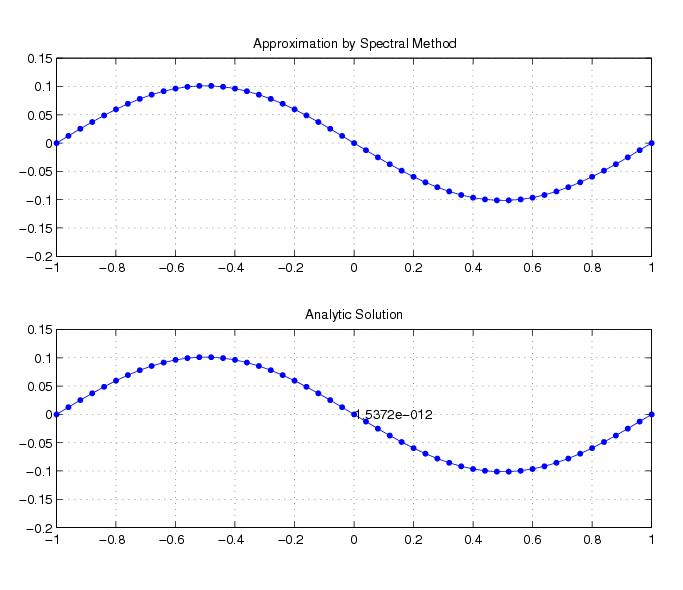
\epsfig{file = Doc-Report_Fwd1D/figs_dn/sinDN_O15.eps, width = 5cm}
    \caption{\label{sinsol1}Numerical and exact solution of equation (\ref{pois_sin1}) with polynomial order $P=15$}
    \end{center}
\end{figure}

\subsubsection {H/P Convergence Test for One-dimensional Solution}

\begin{figure}[h]
\begin{center}
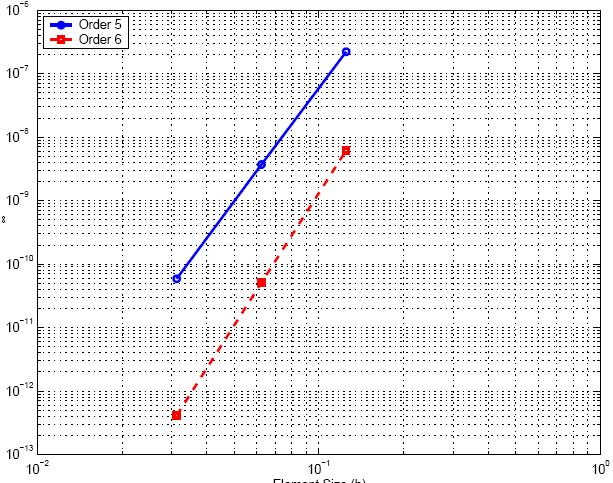
\epsfig{file = Doc-Report_Fwd1D/figs_dn/sinDNhconv.eps, width =8.3cm}
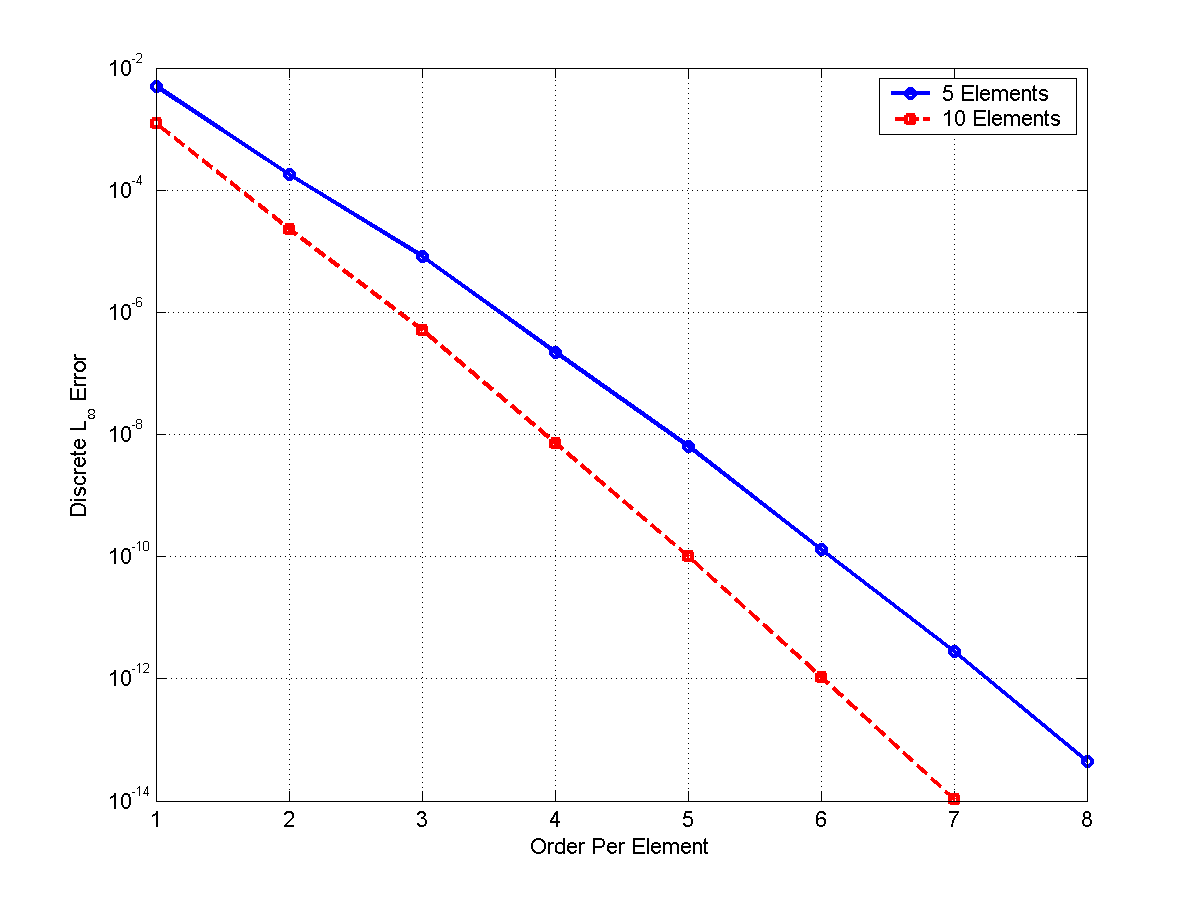
\epsfig{file =Doc-Report_Fwd1D/figs_dn/sinDNpconv.eps,width = 8.3cm}

\caption{\label{sinDNconv1} (Left) Convergence with respect to
discrete $L^{\infty}$ norm as a function of size of elements. This
test is performed using the h-type extension with polynomials of
order 3, 4, and 5 respectively. Error on the Log-Log axis
demonstrates the algebraic convergence of the h-type extension.
(Right) Convergence w.r.t. $L^{\infty}$ norm as a function of size
of polynomial order in semi-Log plot. This shows the exponential
convergence of p-type extension for smooth solution. The tests
were performed for p-type extension with element length $0.2$ and
$0.1$. }
\end{center}
\end{figure}
In this section we present the result of convergence in both $h$
refinement and $p$ refinement with the following steady-state
Poisson differential equation:
\begin{equation}
\label{pois_sin1} \frac{d^2}{dx^2} u(x) = \sin(\pi x),
\end{equation}
for all x in $[-1, 1]$ with zero Dirichlet and Neumann boundary
conditions.


For comparison, the numerical and exact solutions are depicted in
figure (\ref{sinsol1}).

\begin{enumerate}

\item {Convergence of h-type extension for equation (\ref{pois_sin1})}

This test seeks to establish the relation between size of element
and the accuracy of approximation. Utilizing equi-distance
elements, we investigate error. As shown in Figure
(\ref{sinDNconv1}), as elements decrease in size, the accuracy of
the solution improves.

As we see the relationship (\ref{hrelation}) in the theory, the
slope of convergence graph should exhibit slopes of slope 4, 5,
and 6 for the polynomial orders 3, 4, and 5, respectively. The
exact outcome is shown in left table of Table (\ref{hconv2t1}).

\item {Convergence of p-type extension for equation (\ref{pois_sin1})}

Since the exact solution is an infinite sum of polynomial
function, finite order interpolating trial functions cannot reach
ideal convergence. It is also apparant that the convergence will
stagnate before the error reaches machine precision, shown in
right figure of Figure (\ref{sinDNconv1}), the experimented
results support the behavior described in equation
(\ref{hprelation}).

\end{enumerate}

\begin{table}[h]
\centering \caption{\label{hconv2t1} This table shows the
convergence of h-type (left) and p-type (right) resolution control
done above Figure (\ref{sinDNconv1}). Observe that the slopes of
each order $P$ is $P+1$. }
\begin{tabular}{|c|c|c|} \hline
    Polynomial order&Error($L^{\infty}$)&Slope   \\ \hline \hline
    3&$1.1620e-012$ &$4.0024$ \\ \hline
    4&$4.6629e-014$ &$4.9877$ \\ \hline
    5&$9.7367e-014$ &$5.9775$ \\ \hline
\end{tabular}
\hspace{.5in}
\begin{tabular}{|c|c|} \hline
    &\multicolumn{1}{|c|}{Error}\\
    \raisebox{0.5\baselineskip}%
    {Element Size}&($L^{\infty}$) \\ \hline \hline
    0.2&$8.3267e-016$  \\ \hline
    0.1&$6.6613e-016$  \\ \hline
\end{tabular}

\end{table}

%\subsection {Approximation of High order Polynomial solving
                                                1-D Poisson Equation}

In this section we construct a polynomial $P_n$ of order $n$
defined on $[0,1]$, which satisfies the following.
\begin{eqnarray*}
 P_n(0) = 0, &P_n(1) = 1 \\
 \frac{d^k}{dx^k}P_n(0) = 0, &\frac{d^k}{dx^k}P_n(1) = 0
\end{eqnarray*}
for all $k = 1, \cdots, n-2$. \\
Then for each $n$, we obtain a polynomial $P_n$ by solving a
system of linear equations having unique solution which determines
the set of coefficients of $P_n$. We will apply the spectral
polynomial solver to approximate the second derivative $Q_{n-2}$
of $P_n$.

Figure \ref{sol1} is showing some samples of solution of
order($n$) $21$.

\begin{problem}
\label{problem2}Consider the following differential equation for
$u(x)$ such that
\begin{equation*}
    \frac{d^2}{dx^2} u(x) = Q_{n-2},
\end{equation*}
for all $x$ in $[0, 1]$. Then the problem is to find approximation
$p(x)$ of $u(x)$ using spectral polynomial method.
\end{problem}

\noindent
%\begin{minipage}[b]{.46\linewidth}
\begin{figure}
  \centering%
  \epsfig{file = figs/0_sol21.eps, %
        height = 6cm}
  \caption{\label{sol1}Solution polynomial of order 21}
%\end{minipage}\hfill
\end{figure}


\subsubsection{Existence of Approximate Solution}

The Figure \ref{crvconvf1} and \ref{crvconvf2} are showing the
result of spectral polynomial method approximating the solution of
Problem \ref{problem2}. The maximum error value in Table
 \ref{crvconv1t} is showing the approximation is within numerically
exact solution tolerance.

\begin{figure}[h]
\begin{center}
\epsfig{file = figs/3_apcrv_app.eps, %
        height = 9cm}
\caption{\label{crvconvf1}Graph showing spectral approximation
satisfying Problem \ref{problem2}}
\end{center}
\end{figure}

\begin{figure}[h]
\begin{center}
\epsfig{file = figs/3_apcrv_err.eps, %
        height = 9cm}
\caption{\label{crvconvf2}Graph showing the error of approximation
in Figure \ref{crvconvf1}}
\end{center}
\end{figure}

\begin{table}[h]
\centering \caption{\label{crvconv1t} Specification of
                              Figure \ref{crvconvf1} and its error}
\begin{tabular}{|c|c|c|c|} \hline
Element Size &Num. of Element &Orders    &Err   \\ \hline \hline
$0.2$        &$5$             &$5, 5, 5, 5, 5$ &$5.7732e-015$ \\
\hline
\end{tabular}
\end{table}


\clearpage
%----------------------------------------------------------------------

\subsubsection{Convergence of Solution in Equidistance and
Uniformly Ordered Elements}

In this section we show the convergence of solutions obtained by
handling orders of basis on each element. We fix the element to be
same size(length) and divide the domain $[0, 1]$ by 5 elements.

Figure \ref{crvconvf3} is the result of convergence to
approximating to a solution of order $5$ in Problem
\ref{problem2}. It shows monotonic decreasing with same similar
slope until the order reaches from $1$ to $4$, and the slope get
stiff between order $4$ and $5$.

Figure \ref{crvconvf4} is that of solution of order $7$. In this
case, the error stops to decrease after the order is larger than
$7$. This part should be considered carefully and need to be made
sure the applicable range of the numerical method.

\begin{figure}[h]
\begin{center}
\epsfig{file = figs/31_equiconv_ord7.eps, %
        height = 9cm}
\caption{\label{crvconvf4}Graph showing convergence of order 7
problem}
\end{center}
\end{figure}

\begin{figure}[h]
\begin{center}
\epsfig{file = figs/explicitdd_od10_int5_10.eps, %
        height = 9cm}
\caption{\label{crvconvf4}Graph showing convergence of order
10(explicit) problem with 5/10 elements}
\end{center}
\end{figure}

%\clearpage
%----------------------------------------------------------------------

\subsubsection{Test of Convergence of Solution in Variable Ordered
Elements}

According to the idea that the solution need to be carefully
approximated specially in the center of the curve, we assign
different orders by the position of elements. I tested 2 cases.
The one is to variate 3 elements in center among 5 elements. The
other is to variate 1 element in the exact center of all elements.

Figure \ref{crvconvf5} is the first case with 3 different orders
at the $2$ ends of elements. Since it is based on the solution of
order $5$, the orders in 3 center elements moves from $1$ to $5$.

Figure \ref{crvconvf6} is the same as Figure \ref{crvconvf5}
except that it is based on solution of order 7 problem and the
orders at the center elements varies from 1 to 7.


\begin{figure}[h]
\begin{center}
\epsfig{file = figs/32_variconv_ordppp5.eps, %
        height = 9cm}
\caption{\label{crvconvf5}Graph showing convergence of order 5
problem}
\end{center}
\end{figure}

\begin{figure}[h]
\begin{center}
\epsfig{file = figs/32_variconv_ordppp7.eps, %
        height = 9cm}
\caption{\label{crvconvf6}Graph showing convergence of order 7
problem}
\end{center}
\end{figure}

Figure \ref{crvconvf7} and Figure \ref{crvconvf8} are the same as
\ref{crvconvf5} and \ref{crvconvf6} except that these have the
element that varies only a center element. The 2 different control
of orders on each element doesn't give out much different error
movement. This means choosing wise orders in each element can save
time of computing since the lower is the order, the faster does
the system solve.

\begin{figure}[h]
\begin{center}
\epsfig{file = figs/32_variconv_ordp5.eps, %
        height = 9cm}
\caption{\label{crvconvf7}Graph showing convergence of order 5
problem}
\end{center}
\end{figure}

\begin{figure}[h]
\begin{center}
\epsfig{file = figs/32_variconv_ordp7.eps, %
        height = 9cm}
\caption{\label{crvconvf8}Graph showing convergence of order 7
problem}
\end{center}
\end{figure}

\{ {\it  sp2d\_ch3\_1.tex} \}

\subsection {H/P Convergence Test for Solution of Two-dimensional Spectral Fourier Method}

In this section we present the result of convergence in both $h$ refinement and $p$ refinement with the following steady-state Poisson differential equation:
\begin{equation}
\label{pois_sin2}
\frac{d^2}{dr^2} u(r, \theta) + \frac{1}{r} \frac{d}{dr} u(r,\theta) + \frac{1}{r^2} \frac{d^2}{d\theta^2} u(r, \theta)= f(r, \theta),
\end{equation}
for all r in $[a, b], a > 0$ and $\theta$ in $[-\theta, \theta]$ with Dirichlet condition on $a$, and Neumann boundary condition on $b$.

For a periodic function $u(r, \theta) = sin(r)cos(\theta)$, by computation above, we obtain the force function as follows:

\begin{equation}
f(r, \theta) =  \frac{1}{r^2}\left[\{(\frac{2\pi r}{l})^2+1\}\sin S_r - \frac{2 \pi r}{l}\cos S_r \right]\cos\theta.
\end{equation}
where $S_r = 2 \pi \frac{r-a}{l} -\pi$.

The numerical solution by the solver is shown in figure (\ref{sinsol2}).

\begin{figure}[h]
    \begin{center}
    \epsfig{file = figs2_dn/SolSinP15.eps, width = 5cm}
    \caption{\label{sinsol2}
    Numerical and exact solution of equation (\ref{pois_sin}) with polynomial order $P=15$}
    \end{center}
\end{figure}


\begin{itemize}

\item {Convergence of h-type extension for equation (\ref{pois_sin})}

This test is to validate the relation between size of element and the accuracy of approximation. We apply equi-distance elements and investigate the movement of error scale. As shown in Figure (\ref{sinDNconv}), the smaller are the elements, the more exact is the solution.

As we see the relationship (\ref{hrelation}) in the theory, the slope of convergence graph shows slope 4, 5, and 6 for the polynomial order 3, 4, and 5 respectively. the exact outcome is shown in left table of Table (\ref{hconv2t}).

\item {Convergence of p-type extension for equation (\ref{pois_sin})}

Since the exact solution is infinite sum of polynomial function, with finite order of interpolating trial functions cannot reach the ideal convergence. But conversely, this also shows the fact that the convergence stay in steady state before the error reached the machine precision range. As shown in right figure of Figure (\ref{sinDNconv}), it proves the fact that is explained in equation (\ref{hprelation}).

\end{itemize}

\begin{figure}[h]
\begin{center}
\epsfig{file = figs2_dn/sin2DNhconv.eps, width = 6.0cm}
\epsfig{file = figs2_dn/sin2DNpconv.eps, width = 6.0cm}
\epsfig{file = figs2_dn/sin2DNthconv.eps, width = 6.0cm}
\caption{\label{sinDNconv}
(Left)Convergence with respect to discrete $L^{\infty}$ norm as a function of size of elements. This test is performed using the h-type extension with fixed polynomial order 3, 4, and 5 respectively. Error on the Log-Log axis is demonstrating the algebraic convergence of the h-type extension.
(Right)Convergence w.r.t. $L^{\infty}$ norm as a function of size of polynomial order in semi-Log plot. It shows the exponential convergence of p-type extension for smooth solution. Two tests are performed for p-type extension with element length $0.2$ and $0.1$.
}
\end{center}
\end{figure}

\begin{table}[h]
\centering \caption{\label{hconv2t} This table shows the convergence of h-type (left) and p-type (right) resolution control done above Figure (\ref{sinDNconv}). We can see the slopes of each order $P$ is $P+1$ }
\begin{tabular}{|c|c|c|} \hline
    Polynomial order&Error($L^{\infty}$)&Slope   \\ \hline \hline
    5&$5.9175e-014$ &$5.4606$ \\ \hline
    6&$3.0365e-014$ &$6.9478$ \\ \hline
\end{tabular}
%\hspace{.5in}
\begin{tabular}{|c|c|} \hline
    Element Size&Error($L^{\infty}$)  \\ \hline \hline
    0.2&$3.9347e-014$  \\ \hline
    0.1&$7.9098e-015$  \\ \hline
\end{tabular}

\begin{tabular}{|c|c|c|} \hline
    No.Elements&Order&Error($L^{\infty}$)  \\ \hline \hline
    $2^3$&$8$&$3.2580e-012$  \\ \hline
    $2^3$&$9$&$6.4393e-014$  \\ \hline
    $2^3$&$10$&$4.6629e-015$  \\ \hline
\end{tabular}
\end{table}

\{ {\it  sp1d\_ch3\_2.tex} \}

\subsection {High order Polynomial Solution and Its Convergence}

In this section we construct a polynomial $P_n$ of order $n$ defined on $[0,1]$, which satisfies the following.
\begin{eqnarray}
\label{pois_scrv}
    P_n(0) = 0, &P_n(1) = 1 \\
    \frac{d^k}{dx^k}P_n(0) = 0, &\frac{d^k}{dx^k}P_n(1) = 0
\end{eqnarray}
for all $k = 1, \cdots, n-2$. \\
Then for each $n$, we obtain a polynomial $P_n$ by solving a system of linear equations having unique solution which determines the set of coefficients of $P_n$. We will apply the spectral polynomial solver to approximate the second derivative $Q_{n-2}$ of $P_n$.
The numerical and exact solutions by the solver we developed is shown in figure (\ref{scrvsol}).


\begin{figure}[h]
    \begin{center}
 %   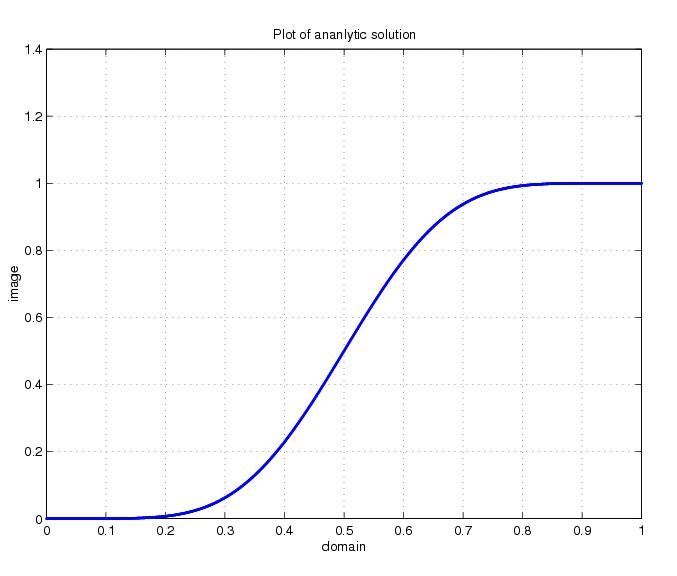
\epsfig{file = figs2_dn/ScrvO_13.eps, width = 5cm}
    \caption{\label{scrvsol}Example of curve that satisfies conditions (\ref{pois_scrv}) with polynomial order $n=13$}
    \end{center}
\end{figure}
We will investigate the convergences by the h-type, p-type extension of trial functions below.

\begin{problem}
Consider the following differential equation for $u(x)$ such that
\begin{equation}
\label{poi_poly}
    \frac{d^2}{dx^2} u(x) = Q_{n-2},
\end{equation}
for all $x$ in $[0, 1]$ with the boundary condition defined in equation (\ref{pois_scrv}). Then the problem is to find approximation $u^{\delta}(x)$ of $u(x)$ using spectral polynomial method.
\end{problem}

Note that the accuracy of this interpolation satisfying equations (\ref{pois_scrv}) is dependent on the stability of matrix that defines the coefficients of interpolants. We used the Legendre basis function which is known to be more stable than monomials. In spite of this, there exists interpolation error close to $e^{-13}$. This cause the same amount of convergence error in p-type extension mode shown in right of Figure (\ref{ScrvconvDN}) and Table (\ref{hconv2t}).

\begin{itemize}

\item {Convergence h-type extension for equation (\ref{poi_poly})}

As we've seen in the case of equation (\ref{pois_sin}), in Figure (\ref{ScrvconvDN}), we see the error with respect to $L^{\infty}$ of the discrete solution to the equation is exponentially convergent to the size of element. This verifies the Log-Log scale of relation of theory (\ref{hrelation}).

\item {Convergence p-type extension for equation (\ref{poi_poly})}

This semi-Log scale plot also showing the exponential convergence of p-type extension of trial functions. Note that we approximate the finite order of polynomial. So there exists the lowest order $P_l$ that approximating with trial functions of order $P$ which $P > P_l$ should shows the same convergence as the case using trial functions of order $P_l$. In right of Figure (\ref{ScrvconvDN}), we can see the convergence is staying on approximation error which theoretically should be machine precision.

\end{itemize}

\begin{figure}[h]
\begin{center}
%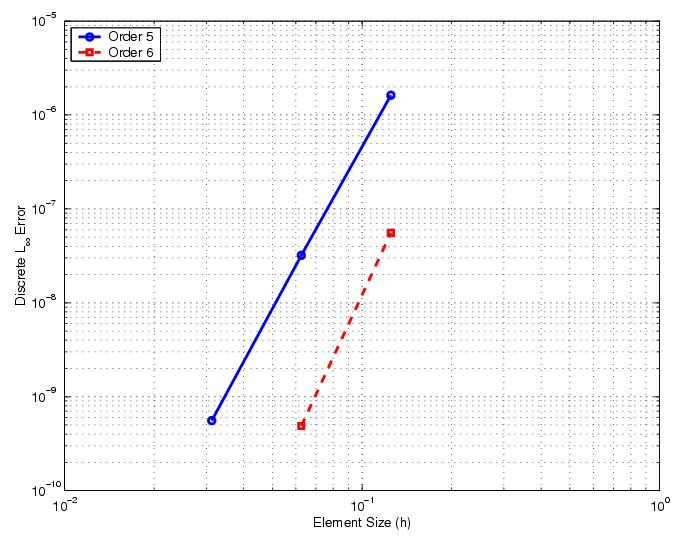
\epsfig{file = figs2_dn/ScrvHconv.eps, width = 8.3cm}
%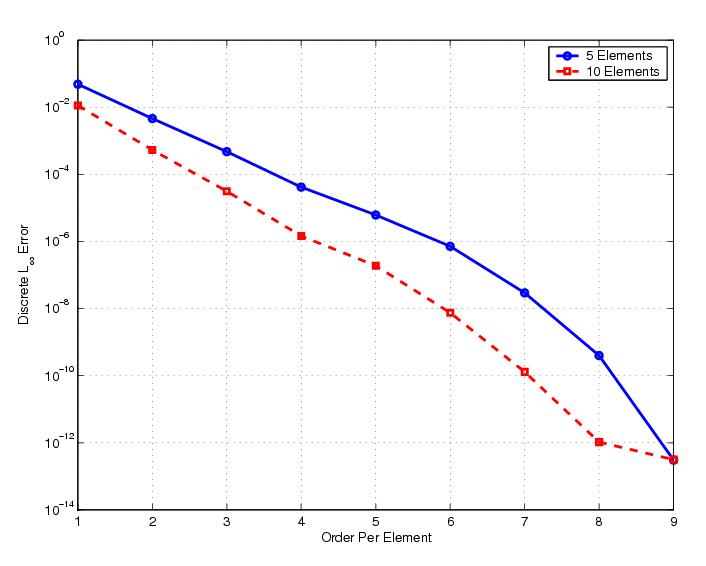
\epsfig{file = figs2_dn/ScrvPconv.eps, width = 8.3cm}
\caption{\label{ScrvconvDN}
(Left)Convergence with respect to discrete $L^{\infty}$ norm as a function of size of elements. This test is performed using the h-type extension with fixed polynomial order 3, 4, and 5 respectively. Error on the Log-Log axis is demonstrating the algebraic convergence of the h-type extension.
(Right)Convergence w.r.t. $L^{\infty}$ norm as a function of size of polynomial order in semi-Log plot. It shows the exponential convergence of p-type extension for smooth solution. Two tests are performed for p-type extension with element length $0.2$ and $0.1$.
}
\end{center}
\end{figure}

\begin{table}[h]
\centering \caption{\label{hconv2t} This table shows the convergence of h-type resolution control done above Figure (\ref{ScrvconvDN}). We can see the slopes of each order $P$ is $P+1$ }
\begin{tabular}{|c|c|c|} \hline
    Polynomial order&Error($L^{\infty}$)&Slope   \\ \hline \hline
    3&$7.5530e-011$ &$3.9908$ \\ \hline
    4&$4.5619e-013$ &$4.6486$ \\ \hline
    5&$4.1855e-013$ &$5.7218$ \\ \hline
\end{tabular}
\hspace{.5in}
\begin{tabular}{|c|c|} \hline
    &\multicolumn{1}{|c|}{Error}\\
    \raisebox{0.5\baselineskip}%
    {Element Size}&($L^{\infty}$) \\ \hline \hline
    0.2&$3.0431e-013$  \\ \hline
    0.1&$3.1186e-013$ \\ \hline
\end{tabular}
\end{table}


\section{Conclusion}
%%\clearpage
%\{ {\it  sp1d\_ch4\_1.tex} \}

Throughout this project, we looked into the theory of Spectral Polynomial Element Method and its solvability. We also investigated the feature of convergence in the viewpoint of h/p convergence property in comparison to classical finite element method. By using Galerkin method, we could incorporate the weak solution and get the problem to be changed to system of linear equations which we can solve it by computer.

By implementing the Spectral element solver for one dimensional
Poisson equation having Dirichlet and Neumann boundary conditions,
we could experiment all the theory with various specific cases of
high-order solutions which were hard to get acceptable convergence
in a given time and resolution of domain.

For the future study, we would like deal with problems regarding:

\begin{itemize}
\item
developing the solver to be applicable to problems defined on special domain by expanding the solver to multi-dimensional one.
\item
based on the theory of Spectral Element Method, doing research about various natural phenomena which we can understand it by a specific mathematical modelling.
\item
utilizing the method in the problem which is ill-posed. By using certain technique that we can approximate the solution, we can also apply this method to the problem and compare with other method in that situation.
\end{itemize}


%-------------------------------------------------------------------------------

%\clearpage

%------------------------------------------------------------------------------
%   BIBLIOGRAPHY
%%\clearpage

%\{ {\it  sp1d\_chbib.tex} \}

\begin{thebibliography}{9}

\bibitem{Karniadarkis}{\bf Spectral/Hp Element Methods for Cfd}
        George Em Karniadakis, Spencer J. Sherwin, \/
        Oxford Univ Press, 1999.

\bibitem{Trefethen}{\bf Spectral Methods in MATLAB}
        Lloyd N. Trefethen, \/
        Society for Industrial and Applied Mathematics, 2001.

\bibitem{Johnson}{\bf Lecture note of Advanced Methods in Scientific Computing}
        Christopher R. Johnson, \/
        School of Computing, University of Utah, 2002.


\end{thebibliography}


%-------------------------------------------------------------------------------
%   APPENDIX
%S
%

\{ {\it  sp1d\_chapdx.tex} \}

%\clearpage
\appendix
\section {Gaussian Quadrature Formula}



\end{document}
